\documentclass[journal,12pt,onecolumn,draftclsnofoot,]{IEEEtran}

\usepackage{xr-hyper}
\makeatletter

\newcommand*{\addFileDependency}[1]{% argument=file name and extension
\typeout{(#1)}% latexmk will find this if $recorder=0
\@addtofilelist{#1}
\IfFileExists{#1}{}{\typeout{No file #1.}}
}\makeatother

\newcommand*{\myexternaldocument}[1]{%
\externaldocument[][nocite]{#1}%
\addFileDependency{#1.tex}%
\addFileDependency{#1.aux}%
\addFileDependency{#1.bbl}%
}
\myexternaldocument{main}


\usepackage[parfill]{parskip}

\usepackage[utf8]{inputenc}
\usepackage{amsmath}
\usepackage{amsfonts}
\usepackage{bbding}
\usepackage{amssymb}
\usepackage{array}
\usepackage{multirow}
\usepackage{graphicx}
\usepackage[caption=false,font=footnotesize]{subfig}
\usepackage{algorithm}
\usepackage{algorithmic}
\usepackage{float}
\usepackage[hidelinks]{hyperref}
\newcommand\algorithmicprocedure{\textbf{procedure}}
\newcommand{\algorithmicendprocedure}{\algorithmicend\ \algorithmicprocedure}
\makeatletter
\newcommand\PROCEDURE[3][default]{%
  \ALC@it
  \algorithmicprocedure\ \textsc{#2}(#3)%
  \ALC@com{#1}%
  \begin{ALC@prc}%
}
\newcommand\ENDPROCEDURE{%
  \end{ALC@prc}%
  \ifthenelse{\boolean{ALC@noend}}{}{%
    \ALC@it\algorithmicendprocedure
  }%
}
\newenvironment{ALC@prc}{\begin{ALC@g}}{\end{ALC@g}}
\makeatother

\usepackage{color}
\usepackage{cite}

\allowdisplaybreaks
\renewcommand{\thefootnote}{\arabic{footnote}}
\DeclareMathOperator{\sgn}{\bf sgn}
\DeclareMathOperator{\cov}{\bf cov}
\DeclareMathOperator{\dom}{\bf dom}
\DeclareMathOperator{\var}{\bf var}
\DeclareMathOperator{\svd}{\bf svd}
\DeclareMathOperator{\expt}{\mathbb{E}}
\DeclareMathOperator{\vari}{\mathbb{V}}
\DeclareMathOperator{\proj}{\textrm{proj}}
\DeclareMathOperator{\gram}{\bf gram}
\DeclareMathOperator{\diag}{\bf diag}
\DeclareMathOperator{\Tr}{\bf Tr}
\DeclareMathOperator{\nsl}{\bf nsl}
\DeclareMathOperator*{\argmax}{\arg\!\max}

% \DeclareMathOperator{\inf}{\bf inf}

%\renewcommand{\baselinestretch}{1.0}
\usepackage{amsthm}
\usepackage{stfloats}
\newtheorem{defi}{Definition}
\newtheorem{theorem}{Theorem}
\newtheorem{lemma}{Lemma}
\newtheorem{condition}{Condition}
\newtheorem{assumption}{Assumption}
\newtheorem{rem}{Remark}
\newtheorem{pro}{Property}
\newtheorem{prop}{Proposition}
\newtheorem{cor}{Corollary}
\newcommand{\red}[1]{{\color[rgb]{1,0,0}{#1}}}
\newcommand{\blue}[1]{{\color[rgb]{0,0,1}{#1}}}
\newcommand{\purple}[1]{{\color[rgb]{0.65,0,0.5}{#1}}}


\usepackage{silence}
\WarningFilter{latex}{Label}

\renewcommand{\label}[1]{}

\title{\Large \textbf{Response Letter of Manuscript TCOM-TPS-26-0080}\\
{\Large Joint Laser Inter-Satellite Link Matching and Traffic Flow Routing in LEO Mega-Constellations via Lagrangian Duality}}
\author{
\IEEEauthorblockN{Zhouyou Gu, Jinho Choi, Jihong Park}\\
\thanks{Decision letter received on 21-Mar-2026.}}



\begin{document}

\maketitle

The manuscript was previously rejected based on three reviewer reports; however, after careful examination, it became evident that the comments from Reviewer 2 were irrelevant to the submitted work and appeared to review a different paper. In contrast, the reports from Reviewers 1 and 3 were relevant and constructive, and we have carefully addressed their comments through a thorough revision. Following guidance from the IEEE Transactions on Communications editorial team, we are therefore resubmitting the revised manuscript as a new submission representing a major revision of the original work.

We summarize the substantive revisions below so that the changes can be evaluated on their own merits without requiring the original review history. Detailed point-by-point responses to the relevant comments from Reviewers 1 and 3 are provided in the subsequent sections, and the revised text is highlighted in blue for easy reference.

\begin{itemize}

\item \textbf{Step-by-step NP-hardness proof.} The fixed-snapshot abstract decision problem, abstract snapshot joint matching and routing (AS-JMR), was introduced, NP-hardness was stated as Proposition~\ref{prop:np_hardness}, and a new appendix proves it through a step-by-step reduction from integral 2-commodity flow in symmetric digraphs. A remark in the main text explains the precise scope of the hardness statement and why it does not by itself imply NP-hardness of the full geometric/orbital formulation.

\item \textbf{Convergence statement clarified.} The dual convergence guarantee was restated in terms of the best-so-far dual iterate, transient subgradient oscillations on bottleneck links were explained, and the simulation discussion was adjusted so that it no longer implies monotone per-iteration improvement.

\item \textbf{Stronger baseline set.} The baseline set was strengthened to include a deep reinforcement learning baseline (DRL), a non-joint traffic-engineering baseline (SaTE), a maximum-rate matching baseline (MRate), and a grid-based matching baseline (``+Grid''), all compared against the proposed DuJo. The previous random-matching baseline is retained as supporting context only.

\item \textbf{More realistic simulation setup.} A coherent shell-tracking benchmark on a deterministic Starlink shell across multiple snapshot offsets and a load-stress benchmark across eight load levels were added under the strengthened baseline set. The previous random-subset evaluation is retained as a separate scale study.

\item \textbf{Pointing-jitter assumption removed.} The i.i.d.\ assumption on pointing errors across LCTs was removed from the system model. Each LCT is now characterized only by its marginal Rayleigh jitter distribution, which is all that the per-link capacity derivation requires, so per-LCT jitter scales can be accommodated without changing the matching or routing algorithm.

\item \textbf{Acquisition-and-tracking scope made explicit.} The original ideal-acquisition wording was replaced with an explicit per-snapshot scope statement and an acknowledged acquisition, pointing, and tracking (ATP) limitation, and a new appendix formalizes an ATP-aware Markov decision process (MDP) extension and shows that our three-way Lagrangian decomposition is preserved at each snapshot.

\item \textbf{LCT visibility model formalized.} The relevant subsection was renamed to ``LCT Visibility and Connection Constraints,'' an explicit connectable-pair condition built from the maximum-distance bound and the mutual field of regard test was added, both intra-plane and inter-plane LISLs are now explicitly admitted whenever the geometric condition is satisfied, and a scope note on atmospheric and Earth-occlusion effects was added.

\item \textbf{Traffic-profile scope tightened.} The high-level claim was narrowed to a snapshot-level spatial traffic profile, the omission of temporal variation and purchasing-capability effects was acknowledged, and inline citations to richer demand-modeling directions were added.

\item \textbf{Gateway capacity terminology clarified.} The variable $Q$ is now stated explicitly as the gateway service capacity between a gateway-connected satellite and the terrestrial Internet, distinguished from LISL transit capacity, and ``gateway'' terminology is used consistently across the notation table and the simulation setup.

\item \textbf{Deployment scope clarified.} The optimization is now framed as a centrally orchestrated per-snapshot planner carried out by the ground or network-control segment, and practical deployment challenges including control-plane latency, imperfect traffic and state estimates, robustness to disturbances, and hierarchical or distributed control are discussed as future directions.

\item \textbf{Focused writing cleanup.} A focused proofreading pass was applied to the introduction, notation paragraph, LCT-mechanics exposition, simulation discussion, complexity discussion, and conclusion, including the correction of typographical errors.
\end{itemize}

We believe that these revisions substantially strengthen the manuscript, and we hope that the revised manuscript will now meet the standards for publication in IEEE Transactions on Communications.

\section*{\centering\Large\textbf{Response to Reviewer 1 of Manuscript TCOM-TPS-26-0080}}

\textbf{Comment 1: Is the assumption of independent and identically distributed pointing errors across LCTs realistic in practical satellite platforms?}

\textbf{Response:} We thank the reviewer for raising this point. We agree that strict statistical independence and identical distribution of pointing errors across LCTs are simplifications that may not hold on practical multi-LCT platforms, where jitter can be correlated through shared attitude and control dynamics, and per-terminal jitter scales can differ when terminals are not identically calibrated \cite{kaymak2018survey,yang2024analysis}. Accordingly, the i.i.d.\ assumption was removed from the manuscript. Each LCT's pointing jitter is now characterized only by its marginal Rayleigh distribution, and the per-link capacity derivation depends only on this marginal. Per-LCT jitter scales can therefore be accommodated without changing the matching or routing algorithm.

\textbf{Manuscript changes:} The previous i.i.d.\ statement was replaced with a marginal-distribution statement in the system model as follows:

``\dots\blue{Each LCT's pointing error is characterized by the marginal Rayleigh distribution above. Since the per-link capacity derivation in the next subsection depends only on each LCT's marginal distribution \cite{kaymak2018survey,yang2024analysis}, the framework does not require pointing errors to be statistically independent or identically distributed across LCTs, and per-LCT jitter scales can be accommodated without changing the matching or routing algorithm.}''

\textbf{Comment 2: Why is the acquisition and tracking time loss strictly assumed to be zero? To the best of my knowledge, LCT alignment in practical satellite systems incurs non-negligible time overhead.}

\textbf{Response:} We agree with the reviewer. Zero acquisition and tracking loss is not a realistic operational assumption for practical optical inter-satellite links \cite{kaymak2018survey,li2011analytical,scheinfeild2000acquisition}. In the revised manuscript, we therefore no longer present it as an ideal physical condition. Instead, we state explicitly that the present formulation is a per-snapshot optimization at a fixed time $t$, so it optimizes the matching, routing, and rate allocation within one snapshot but does not model the time overhead caused by changing LCT alignments across consecutive snapshots. This is a scope limitation, especially when snapshot intervals are short. To make the limitation clear, we revised the system model to acknowledge ATP overhead directly and added an appendix that outlines how an ATP-aware extension could be formulated as an MDP for future work.

\textbf{Manuscript changes:} We have replaced the ``ideal acquisition and tracking'' wording with an explicit per-snapshot scope, an ATP limitation statement, and the MDP extension as follows:

``\dots\blue{Our formulation performs per-snapshot joint design of the matching, routing, and rate allocation at a fixed time $t$, and does not model acquisition, pointing, and tracking (ATP) overheads that arise when the matching changes across snapshots \cite{kaymak2018survey,li2011analytical,scheinfeild2000acquisition}. At short snapshot intervals on the order of seconds, ATP overheads are not negligible, which we acknowledge as a scope limitation of this work. An ATP-aware extension can be cast as a Markov decision process (MDP) on the matching state in which our current three-way Lagrangian decomposition is preserved at each snapshot; details are provided in the appendix. The present formulation corresponds to the degenerate case with zero ATP time, and the full MDP extension is left as future work.}''

We have also added a new appendix ``An MDP Extension for Future Work'' to outline the ATP-aware formulation and to show that the present paper is recovered as the degenerate ATP-free case.

\textbf{Comment 3: You’d better provide a step-by-step mathematical reduction for the NP hardness proof.}

\textbf{Response:} We thank the reviewer for this comment, and the reviewer was right that the original NP-hardness discussion was too terse to support the claim rigorously. We therefore added a step-by-step reduction from integral 2-commodity flow in symmetric digraphs \cite[Theorem 1]{jarry2012multiflows} to the fixed-snapshot abstract decision problem, abstract snapshot joint matching and routing (AS-JMR). The source instance consists of a symmetric directed graph with two integral commodities, capacities $\kappa(u,v)$, demands $d_1,d_2$, and total demand $D=d_1+d_2$. From it, we construct an AS-JMR instance by creating the original graph vertices as satellites, adding one source-terminal and one target-terminal satellite for each unit demand, setting the AS-JMR throughput threshold to $\zeta=D$, creating one unit-rate dedicated LCT pair for each unit of source-arc capacity, and adding attachment LCT pairs from each unit source terminal to its commodity source and from its commodity target to the corresponding unit target terminal. Isolated LCTs are added only to equalize the number of LCTs per satellite and do not create extra connectable pairs.

The equivalence is then shown in both directions. If the source instance has feasible integral 2-commodity flows, decomposing those flows into unit paths gives one feasible AS-JMR route for each unit-demand terminal pair, and the dedicated LCT pairs provide exactly the copied arc capacities, so AS-JMR attains throughput $D=\zeta$. Conversely, if the constructed AS-JMR instance attains throughput at least $D$, then all $D$ unit-demand variables must equal one. Each corresponding binary routing vector contains a unit path from its added source terminal to its added target terminal; deleting the two attachment arcs yields an original $s_h$--$t_h$ path. Because only $\kappa(u,v)$ dedicated unit-rate LCT pairs exist between any adjacent original satellites, aggregating the extracted paths respects the original arc capacities and gives feasible integral 2-commodity flows. The construction is polynomial because the hard source family has polynomially bounded demands and capacities in $\{1,2,3\}$, and the isolated-LCT padding is also polynomial.

We state Proposition \ref{prop:np_hardness} for AS-JMR, rather than directly for the full physical formulation \eqref{eq:prob:constrainted_routing_and_matching:primal}, because the reduction fixes the combinatorial snapshot input instead of deriving it from the geometry, field of regard constraints, distance thresholds, and traffic-pair construction rules. Thus, the proposition, the scope clarification in the main text, and the appendix proof are aligned.


\textbf{Manuscript changes:} Outside the appendix, we revised the abstract, introduction, contribution summary, problem-formulation section, and conclusion. The revised text read as follows:

In the abstract, we stated:

``\dots\blue{The resulting per-snapshot formulation is a mixed-integer program coupling LCT connections with flow-rate variables under link capacity constraints, and the associated fixed-snapshot abstract decision problem is proved to be NP-hard.}''

We revised the introduction as follows.

``\dots\blue{The joint link-matching and flow-routing formulation leads to a mixed-integer optimization problem \cite{ahuja1993network}, and the associated fixed-snapshot abstract decision problem is NP-hard \cite{jarry2012multiflows} (as proved later in Proposition~\ref{prop:np_hardness} and the appendix).}''

In the transition to the method section, we stated:

``\dots\blue{To tackle this mixed-integer problem, we apply the Lagrangian dual relaxation method by lifting the maximum rate limitation constraints between neighboring satellites via Lagrange multipliers.}''

In Contribution 1, we stated the additional complexity result as follows:

``\dots\blue{We provide a comprehensive formulation of the problem \eqref{eq:prob:constrainted_routing_and_matching:primal}, including the LCTs' steering ranges and vibrations, and the diverse traffic profile across the constellation. Moreover, we discuss the complexity of the joint problem through the induced fixed-snapshot abstract decision problem. Specifically, we define this abstract decision problem and prove that it is NP-hard, via a direct reduction from integral 2-commodity flow in symmetric digraphs \cite{jarry2012multiflows}.}''

In the paragraph introducing the complexity formulation, we stated:

``\dots\blue{Problem~\eqref{eq:prob:constrainted_routing_and_matching:primal} is the physical mixed-integer formulation built from the geometric/orbital system model. To analyse its hardness, we fix one snapshot and abstract away the geometric/orbital derivation of the connectable pairs, the source-target pair set, and the link rates. This yields the following fixed-snapshot abstract decision problem, to which Proposition~\ref{prop:np_hardness} with its proof in the appendix applies.}''

Immediately after the problem formulation, we inserted the following non-appendix block:

{\color{blue}
\begin{defi}[AS-JMR]
The abstract snapshot joint matching and routing (AS-JMR) decision problem has input
\begin{equation}
  \begin{aligned}
    (\mathcal{I},\mathcal{N},\{i_n\}_{n\in\mathcal{N}},\mathcal{E},\mathcal{F},\{r_{n,m}\}_{\{n,m\}\in\mathcal{E}},\{Q_i\}_{i\in\mathcal{I}},\{D_i\}_{i\in\mathcal{I}},\zeta),
  \end{aligned}
\end{equation}
where $\mathcal{I}$ is the satellite set, $\mathcal{N}$ is the LCT set, $i_n\in\mathcal{I}$ is the satellite carrying LCT $n$, $\mathcal{E}$ is the set of connectable LCT pairs, $\mathcal{F}$ is the set of source-target satellite pairs, $r_{n,m}\geq 0$ is the rate of pair $\{n,m\}$, $Q_i\geq 0$ and $D_i\geq 0$ are the serving and demand bounds, and $\zeta\geq 0$ is a threshold. Define
\begin{equation}
  \begin{aligned}
    \mathcal{E}_{i,j} = \big\{\{n,m\}\in\mathcal{E}\big| i_n = i, i_m = j\big\},
    \mathcal{L} = \big\{(i,j)\big| \mathcal{E}_{i,j}\neq \emptyset \big\}.
  \end{aligned}
\end{equation}
The task is to verify the existence of $\mathbf{c}\in\mathcal{C}$, $\mathbf{q}\in\mathcal{Q}$, and $\mathbf{x}\in\mathcal{X}$ satisfying \eqref{eq:const:path:flow_rate} and
\begin{equation}
  \begin{aligned}
    \sum_{(s,s')\in\mathcal{F}} q^{s,s'} \geq \zeta.
  \end{aligned}
\end{equation}
\end{defi}

\begin{prop}\label{prop:np_hardness}
The decision problem AS-JMR is NP-hard.
\end{prop}

\begin{proof}
  The proof is listed in the appendix.
\end{proof}
}

Immediately after Proposition \ref{prop:np_hardness}, we stated:

``\dots\blue{The reduction in Proposition~\ref{prop:np_hardness} fixes the combinatorial snapshot input and proves hardness for the resulting fixed-snapshot abstract decision problem, rather than deriving those objects from the underlying geometry, field of regard constraints, distance thresholds, and traffic-pair construction rules.
A direct NP-hardness claim for~\eqref{eq:prob:constrainted_routing_and_matching:primal} requires mapping AS-JMR instances to the realization of~\eqref{eq:prob:constrainted_routing_and_matching:primal}.
Depending on the geometric/orbital parameters, it is possible that some instances of~\eqref{eq:prob:constrainted_routing_and_matching:primal} are not NP-hard, e.g., when there are no connectable pairs or no source-target pairs.}''

In the sentence immediately following that remark, we stated:

``\dots\blue{Nevertheless, the NP-hardness of AS-JMR implies that the difficulty of the joint link matching and flow routing problem is inherent in the combinatorial nature of the problem, which motivates us to design efficient algorithms based on Lagrangian dual relaxation to solve the problem in the following section.}''

In the conclusion, we stated:

``\dots\blue{It has also shown that the method can be practically computable for this mixed-integer formulation, while the associated fixed-snapshot abstract decision problem is NP-hard and the computing time increases for larger constellations.}''

\textbf{Comment 4: Will the subgradient descent handle potential oscillations when multiple flows compete for the same bottleneck LISLs?}

\textbf{Response:} We agree that subgradient ascent does not guarantee monotone per-iteration behavior when several flows compete for the same bottleneck LISLs. The mathematically correct guarantee is instead on the best-so-far dual value under diminishing step sizes \cite{boyd2003subgradient,boyd2004convex}. Transient oscillations can still occur, but their amplitude is damped asymptotically. We therefore revised the manuscript to state this distinction explicitly, rather than leaving the impression that every iterate is oscillation-free. We further revised the simulation discussion so that it no longer suggests monotone iteration-by-iteration improvement, and both the dual values and the converted throughput may fluctuate when bottleneck links are contested, but these fluctuations become milder as the step size decays.

\textbf{Manuscript changes:} We revised the relevant discussion as follows:

In the subgradient-descent description, we stated:

``\dots\blue{Because several flows may compete for the same bottleneck LISLs, the subgradient iterates need not be monotone: the dual variables and the converted primal solutions can oscillate before settling. The diminishing step size attenuates these oscillations asymptotically, so the convergence guarantee below is stated for the best-so-far dual iterate rather than for every individual iterate.}''

In Theorem \ref{theorem:convergence:classic}, we stated:

{\sloppy
``\dots\blue{Define the best-so-far dual iterate as $\hat{\lambda}^{[k]} \in \argmax_{\lambda^{[i]}:i=1,\dots,k} g(\lambda^{[i]})$ after $k$ iterations. The corresponding dual value converges to the optimal dual value $g(\lambda^*)$ as $k\to\infty$, i.e., $\lim_{k\to\infty} g(\hat{\lambda}^{[k]}) = g(\lambda^*)$. Specifically, the dual-value gap satisfies $g(\lambda^*) - g(\hat{\lambda}^{[k]}) = \mathcal{O}(k^{-(1-\beta)})$ when $0.5\leq\beta<1$.}''\par
}

In the numerical-results discussion, we stated:

``\dots\blue{As expected for subgradient methods, the per-iteration dual values are not necessarily monotone and may fluctuate when multiple flows compete for the same bottleneck LISLs. Nevertheless, the diminishing step size progressively damps these fluctuations, while Theorem \ref{theorem:convergence:classic} concerns the best-so-far dual value rather than every individual iterate.}''

``\dots\blue{The converted throughput can also fluctuate across iterations, but it approaches a stable level as the multipliers settle.}''

\textbf{Comment 5: Why does the evaluation only randomly sample a given number of satellites from the Starlink data instead of simulating a complete structured orbital shell (or multiple shells)?}

\textbf{Response:} We agree that randomly sampled Starlink subsets alone are not sufficient as realistic orbital-geometry evidence. In the revised manuscript, we therefore use random Starlink subsets only for the varying-$I$ and computing-time sensitivity study, where the purpose is to test scaling with constellation size. For the realism-oriented Starlink evaluation, we added a structured-shell study that uses one coherent $I=1000$ satellite block from the dominant $53.2^\circ$ shell and tracks the same satellites over six snapshot times. We did not run a complete Starlink shell or all Starlink shells for every method and snapshot because the repeated multi-method, multi-snapshot comparison would be substantially more expensive. The coherent shell block keeps the evaluation computationally manageable while preserving structured orbital geometry. The manuscript also includes structured-constellation comparisons for a regular Walker-delta case and the OneWeb constellation in Fig. \ref{fig:plot_test_dual_optimization_different_constellation}.

\textbf{Manuscript changes:} In the simulation setup and the numerical-results discussion, we revised the text accordingly. The revised text read as follows.

In the simulation setup, we stated:

``\dots\blue{To study problem-scale sensitivity, we randomly select $I$ satellites out of the Starlink constellation for the varying-$I$ and computing-time results. We also test a structured shell-based Starlink instance with $I=1000$ satellites. Specifically, at $\mathcal{T}_0$ we select a coherent 1000-satellite block from the dominant $53.2^\circ$ shell and then keep the same satellites over snapshot offsets of $0$, $30$, $60$, $90$, $120$, and $180$ min.}''

In Subsubsection~\ref{subsubsec:structured_shell_time_evaluation}, we stated:

``\dots\blue{We next evaluate the structured shell-based Starlink instance. Fig.~\ref{fig:plot_test_tcom_shell_time_baselines} shows the results for the same $I=1000$ satellite block over six snapshot times.}''

For direct inspection, the revised Fig. \ref{fig:plot_test_tcom_shell_time_baselines} is also reproduced in this response letter.

\begin{figure}[H]
\centering
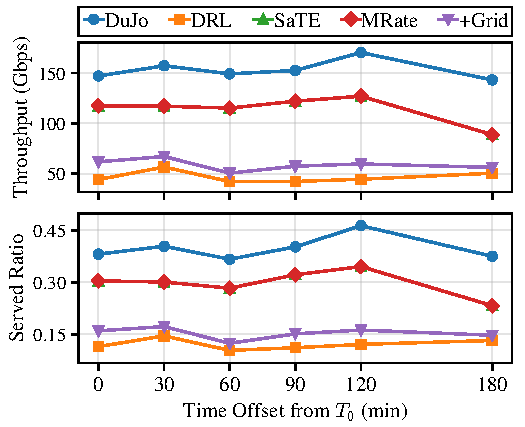
\includegraphics[scale=0.85]{plot_test_tcom_shell_time_baselines.pdf}
\caption{\blue{(Fig. \ref{fig:plot_test_tcom_shell_time_baselines} in the revised manuscript) Structured shell-based Starlink evaluation over time. A coherent $I=1000$ satellite block from the dominant $53.2^\circ$ shell is kept fixed while the constellation is propagated over snapshot offsets of $0$, $30$, $60$, $90$, $120$, and $180$ min. The top plot shows the served throughput and the bottom plot shows the served-demand ratio for DuJo, DRL, SaTE, MRate, and +Grid.}}
\label{fig:resp_plot_test_tcom_shell_time_baselines}
\end{figure}

\textbf{Comment 6: Why are the baseline methods limited to basic heuristics? You may want to include a comparison with recent state-of-the-art schemes to better demonstrate your performance gains.}

\textbf{Response:} We agree that the original baseline set was too weak for the main topology comparison. In the revised manuscript, we therefore strengthened the benchmark by adding the non-joint traffic-engineering baseline SaTE \cite{wu2025sate} and a trained policy-gradient DRL baseline \cite{sutton2000policy}, while retaining MRate and +Grid. At the same time, we demoted the random baseline to supporting context only rather than treating it as a headline practical benchmark. To keep the comparison fair, the added structured-shell study evaluates DuJo, DRL, SaTE, MRate, and +Grid under the same feasible connectability set, the same gateway placement, and the same rate-allocation backend once the matching and routing decisions are fixed.

\textbf{Manuscript changes:} In the baseline-methods subsection, we added the stronger baselines and reduced the prominence of the random baseline. The key revised text read as follows.

In the baseline-methods subsection, we added the following baseline descriptions:

\begin{itemize}
\item \blue{\textbf{SaTE:} Following the non-joint traffic-engineering setting of SaTE \cite{wu2025sate}, this baseline first fixes the LISL matching by maximum link rate matching and then routes the flows by shortest paths under unit hop cost. Given that topology and routing, the traffic flow rates are computed optimally by LP to maximize the network throughput. Thus, only the traffic rate allocation is optimized, while the link matching and traffic routing are not jointly optimized.}
\item \blue{\textbf{DRL:} A trained policy-gradient baseline \cite{sutton2000policy} uses the constellation graph as its state, where each satellite node carries its gateway service capacity and traffic demand and each connectable satellite pair carries its candidate LISL capacity. Its action is to infer the price graph over the connectable satellite pairs, and its reward is derived from the resulting traffic-rate allocation after converting those inferred prices to matching, routing, and rate allocation.}
\end{itemize}

``\dots\blue{In the structured-shell comparison, we focus the main benchmark on DuJo, DRL, SaTE, MRate, and +Grid.}''

For direct inspection, the revised Figs. \ref{fig:plot_test_dual_optimization_vs_grid_rand}, \ref{fig:plot_test_dual_optimization_vs_grid_rand_varying_availability_and_for}, and \ref{fig:plot_test_dual_optimization_different_constellation} are also reproduced in this response letter.

\begin{figure}[H]
\centering
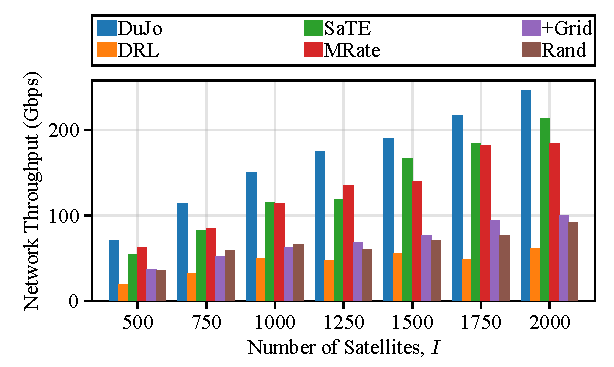
\includegraphics[scale=0.85]{plot_test_dual_optimization_vs_grid_rand.pdf}
\caption{(Fig. \ref{fig:plot_test_dual_optimization_vs_grid_rand} in the revised manuscript) DuJo vs. baselines for different numbers of satellites $I$.}
\label{fig:resp_plot_test_dual_optimization_vs_grid_rand}
\end{figure}

\begin{figure}[H]
\centering
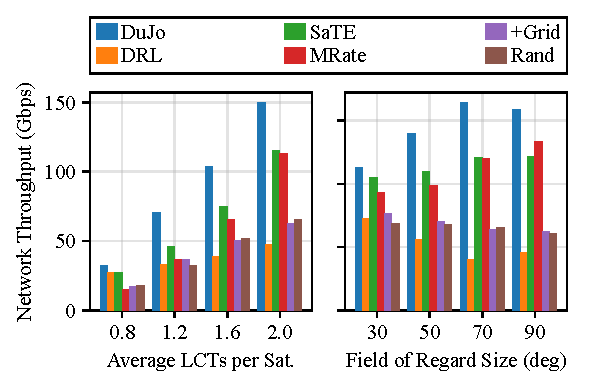
\includegraphics[scale=0.85]{plot_test_dual_optimization_vs_grid_rand_varying_availability_and_for.pdf}
\caption{(Fig. \ref{fig:plot_test_dual_optimization_vs_grid_rand_varying_availability_and_for} in the revised manuscript) Comparison when varying LCT configurations on satellites.}
\label{fig:resp_plot_test_dual_optimization_vs_grid_rand_varying_availability_and_for}
\end{figure}

\begin{figure}[H]
\centering
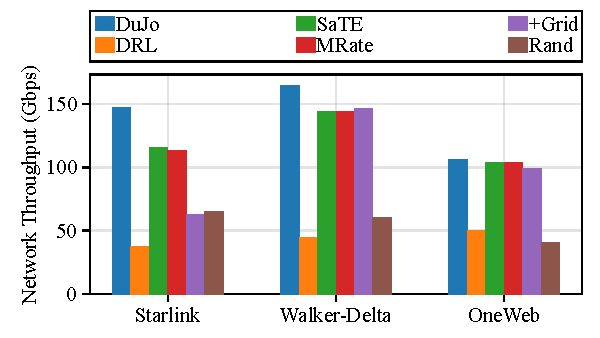
\includegraphics[scale=0.85]{plot_test_dual_optimization_different_constellation.pdf}
\caption{(Fig. \ref{fig:plot_test_dual_optimization_different_constellation} in the revised manuscript) Comparison in a Starlink-based ($I=1000$), a regular walker-delta ($50^{\circ}$ inclination, $I=1000$), and a OneWeb constellation ($I=650$).}
\label{fig:resp_plot_test_dual_optimization_different_constellation}
\end{figure}

These updated figures show that, in the varying-$I$ study, SaTE is generally the strongest separated baseline as the constellation size grows, while DRL remains below the heuristic baselines. In the LCT-configuration and FOR sweeps, DuJo stays strongest across the range, SaTE is generally the strongest separated baseline, and DRL remains lower. In the constellation comparison, DuJo is strongest in all three cases; SaTE is the strongest separated baseline in the Starlink case, while +Grid and SaTE come much closer to DuJo in the walker-delta and OneWeb cases, and DRL remains distinctly lower. This is because the DRL policy is trained using a network-wise reward that is derived from the resulting traffic flow rates, which do not directly supervise how the Lagrange multipliers should be optimized to improve the matching and routing decisions. Thus, the DRL policy may not learn to optimize the Lagrange multipliers effectively, especially when the constellation size grows with many satellite pairs.

\textbf{Comment 7: Paper writing would benefit from improvement. Please also double-check for typos throughout the paper.}

\textbf{Response:} We agree that the writing benefited from tightening. We rechecked the full manuscript for typographical, grammatical, and clarity issues, and then made focused corrections where issues were found. The edits were concentrated in the introduction and notation section, the LCT-mechanics description, figure captions, the simulation discussion, and the conclusion, where several explanatory sentences were awkward or ambiguous. These edits do not change the technical content, but they make the presentation cleaner and easier to follow.

\textbf{Manuscript changes:} We rechecked the full manuscript and made focused writing cleanup edits in the introduction, notation paragraph, LCT-mechanics description, several figure captions, the simulation discussion, and the conclusion.



\section*{\centering\Large\textbf{Response to Reviewer 3 of Manuscript TCOM-TPS-26-0080}}

\textbf{Summary by Reviewer 3: Authors present a method to jointly optimize LCT connections in a satellite constellation to maximize throughput and considering LCT mechanics and global traffic demand. The proposed method is based on a Lagrangian duality based concept to relax the untractability of the joint optimization problem. The method is fully addressed, and authors offer results of complexity. Results are promising compared to the baseline cases, but there are some major concerns that should be addressed to validate performance results.}

\textbf{Response:} We agree that the main validation issues were the explicit visibility model, the scope of the traffic model, the interpretation of the baseline comparisons, and the lack of higher-load evidence. In the revised manuscript, we therefore stated the field-of-regard visibility condition explicitly, clarified the simplified snapshot-level scope of the demand model, corrected the interpretation of gateway service capacity and feasible LISLs, strengthened the baseline comparison with SaTE and DRL, added the structured-shell load-stress evaluation, and clarified the distinction between random Starlink subsets and the structured-shell study. Below, we respond point by point to each comment and identify the corresponding manuscript changes.


\textbf{Comment 1: Authors claim they include mechanical limitations of LCT terminals. However, the only limitation is the FOR range (limited to 60 degrees) and the pointing jitter. In order to validate results, expressions for visibility conditions based on the limited FOR is required and shall be included in the manuscript.}

\textbf{Response:} We agree that the visibility condition should be stated explicitly. In the revised manuscript, this condition was stated directly in Subsection~\ref{subsec:lct_visibility_connection} and formalized in \eqref{eq:lct_visibility_condition}. A potential LISL was treated as admissible only when the inter-satellite distance was within the maximum transmission range and the direction from each LCT to the other satellite lay within that LCT's field of regard. We also stated explicitly that the model does not impose a same-plane restriction, so both intra-plane and inter-plane LISLs can be feasible when they satisfy the same visibility condition. A short limitation note then states that the current connectability approximation does not model atmospheric effects or an explicit line-of-sight or Earth-occlusion constraint.

\textbf{Manuscript changes:} In Subsection~\ref{subsec:lct_visibility_connection}, entitled ``\blue{LCT Visibility and Connection Constraints},'' we revised the wording so that the visibility condition was stated explicitly, the defining condition was given in \eqref{eq:lct_visibility_condition}, the lack of a same-plane restriction was stated explicitly, and the current scope limitation was stated afterward. The key revised text read as follows.

``\dots\blue{The visibility condition for a potential LISL is determined by the maximum beam transmission distance $\hat{z}$ and the mutual field of regard test at the two LCTs.}
\blue{Accordingly, the set $\mathcal{E}$ of all connectable LCT pairs is defined by the following visibility condition.}''
\begin{equation}
  \begin{aligned}
    &\mathcal{E} = \big\{\{n,m\}\ \big| \ i_n \neq i_m, z_{i_n,i_m} \leq \hat{z}, \\
    &\qquad\qquad \mathbf{d}_{i_n,i_m} \cdot \mathbf{u}_n > \cos \theta,\mathbf{d}_{i_m,i_n} \cdot \mathbf{u}_m > \cos \theta \big\}.
  \end{aligned}
\end{equation}
\blue{Therefore, the model does not impose a same-plane restriction. Both intra-plane and inter-plane LISLs can be feasible whenever they satisfy this visibility condition.}
\blue{Note that this visibility model is simplified. We do not model atmospheric effects here because the present LISL formulation focuses on space-to-space propagation. We also do not impose an explicit line-of-sight or Earth-occlusion constraint, so the current connectability approximation is driven only by the range bound and the mutual field of regard test \cite{vallado2022fundamentals,leyva-mayorga2021interplane,yang2024analysis}.}


\textbf{Comment 2: Authors claim the consider global traffic demand. However, the traffic demand model is very basic and does not consider aspects like the purchasing capacibility of the population or temporal variation of the traffic demand. I suggest this reference to refine the traffic model demand: Samuel Martínez Zamacola, Santiago Martín Marco, Ramón Martínez Rodríguez-Osorio, Profiling the transmit power of LEO satellite constellations for broadband communication services considering terrestrial and aerial demand, Acta Astronautica, Volume 236, 2025, Pages 547-559, ISSN 0094-5765, \url{https://doi.org/10.1016/j.actaastro.2025.06.068.}}

\textbf{Response:} We agree that the current traffic model captures only a simplified form of global demand. In the revised manuscript, we stated this scope explicitly. In particular, we clarified that the present demand model is a snapshot-level spatial model driven by the uneven distributions of population and gateways, rather than a full socioeconomic or temporal demand forecast. We also stated directly that the present formulation does not incorporate temporal demand variation or purchasing-capability effects, and we cited richer broadband-demand models for those omitted dimensions, including the terrestrial-and-aerial demand profiling work in \cite{zamacola2025profiling} and the broader broadband-demand model in \cite{qin2024satformer}, together with gateway-aware traffic-estimation work \cite{guo2021gateway}.

\textbf{Manuscript changes:} We narrowed the high-level claim in the abstract and introduction, and in Subsection~\ref{subsec:traffic_profile_model} we stated the simplified scope of the present traffic model explicitly. The key revised text read as follows.

In the abstract, we stated:

``\dots\blue{This paper investigates the joint optimization of LCT connections and traffic routing to maximize the constellation throughput, considering the realistic LCT mechanics and a snapshot-level spatial traffic profile.}''

In the introduction, we stated:

``\dots\blue{Nevertheless, how to design a Lagrangian dual method that considers practical LCT mechanical limitations and a snapshot-level spatial traffic profile over the globe in LEO mega-constellations is still an open problem.}''

In Subsection~\ref{subsec:traffic_profile_model}, we stated:

``\dots\blue{Accordingly, the present traffic model is intended to capture snapshot-level spatial heterogeneity through the uneven distributions of population and gateways, rather than the full demand-forecasting problem.}''

``\dots\blue{This simplified model does not incorporate temporal demand variation or socioeconomic modifiers such as purchasing capability. Richer broadband-demand models along these dimensions are important future work \cite{zamacola2025profiling,qin2024satformer}. Gateway-aware traffic estimation is also relevant to this broader modeling direction \cite{guo2021gateway}.}''


\textbf{Comment 3: Baseline models: authors consider Rand (i.e. random selection of LCT pairs), which is not a proper baseline or benchmark. A rand model would make satellites decide a random ISL link, which is not practical in any sense. Moreover, it should be clarified if in this random selection the limited FOR is considered.}

\textbf{Response:} We agree that random matching is not a proper headline benchmark for practical topology design. In the revised manuscript, we therefore kept Rand only as supporting context and removed it from the main structured-shell comparison, which now focuses on DuJo, DRL, SaTE, MRate, and +Grid. We also clarified that any random matching retained for reference first assigns random weights to the feasible candidate links in $\mathcal{E}$ and then matches the largest weights, so it still respects the same field-of-regard and range constraints as the other methods.

\textbf{Manuscript changes:} In the baseline-methods subsection, we revised the role of Rand and stated its feasibility constraints explicitly. The key revised text read as follows.

In the revised Rand baseline entry, we stated:

\begin{itemize}
\item \blue{\textbf{Rand}: Random matching first assigns random weights to the candidate links in the same feasible connectability set $\mathcal{E}$ and then matches the links from the largest weights. The traffic flows are then routed by OSPF on the resulting topology, where the rates of the paths are allocated by LP.}
\end{itemize}

``\dots\blue{In the structured-shell comparison, we focus the main benchmark on DuJo, DRL, SaTE, MRate, and +Grid.}''


\textbf{Comment 4: Traffic served by a each satellite is quantified as 20 Gbps. It must be declared if this traffic comes from the users or includes ISLs.}

\textbf{Response:} We agree that the traffic accounting should distinguish gateway service capacity from LISL transit capacity. In the revised manuscript, we clarified that $Q$ denotes the per-satellite gateway service capacity between a gateway-connected satellite and the terrestrial Internet. This capacity is used first for the users under that satellite's own coverage, and only the remaining part becomes $Q_i(t)$ for serving other satellites. LISL transit traffic is constrained separately by the capacities of the established optical links and is therefore not already included in $Q=20$ Gbps. We also restated this interpretation in the simulation-setup paragraph.

\textbf{Manuscript changes:} In the traffic profile model and the simulation-setup paragraph, we revised the wording so that gateway service capacity and LISL transit capacity were distinguished explicitly. The key revised text read as follows.

In the traffic profile model, we stated:

``\dots\blue{Here, $Q$ denotes the gateway service capacity available between that satellite and the terrestrial Internet. It does not include LISL transit capacity, which is constrained separately by the aggregate capacities of the established optical links.}''

``\dots\blue{Each satellite first uses this gateway service capacity to serve the traffic demand of its own users under its coverage, i.e., $U_i(t) D$ Gbps for satellite $i$, and then uses the remaining gateway capacity to serve the traffic demand of other satellites.}''

In the simulation setup, we stated:

``\dots\blue{Thus, $Q=20$ Gbps is the per-satellite gateway service capacity before subtracting the traffic of the users under that satellite's own coverage, rather than a limit that already includes LISL transit traffic.}''


\textbf{Comment 5: From the defintion of LCT, it seems that only intraplane ISL are feasible.}

\textbf{Response:} This is not the case in our model. Orbital-plane membership is not itself a feasibility constraint. A pair is admissible whenever its inter-satellite distance is within the range bound and the line-of-sight directions fall within the two LCTs' fields of regard. For that reason, the model does not impose a same-plane restriction, and inter-plane LISLs can also be feasible. In the revised manuscript, we stated this point explicitly in the LCT mechanics, visibility-condition, and simulation-setup text \cite{chaudhry2021laser,leyva-mayorga2021interplane}.

\textbf{Manuscript changes:} We revised the wording so that the fore/aft mounting design is not misread as a same-plane constraint, and we stated explicitly that both intra-plane and inter-plane LISLs may be feasible whenever they satisfy the visibility condition. The key revised text read as follows.

In the LCT mechanics model, we stated:

``\dots\blue{These mounting directions specify only the preferred pointing directions of the LCTs. They do not restrict feasible LISLs to satellites in the same orbital plane \cite{chaudhry2021laser,leyva-mayorga2021interplane}.}''

In Subsection~\ref{subsec:lct_visibility_connection}, we stated:

``\dots\blue{Therefore, the model does not impose a same-plane restriction. Both intra-plane and inter-plane LISLs can be feasible whenever they satisfy this visibility condition.}''

In the simulation setup, we stated:

``\dots\blue{Under this setting, candidate LISLs are not restricted to intra-plane neighbors. Any satellite pair, whether intra-plane or inter-plane, is included if it satisfies \eqref{eq:lct_visibility_condition}.}''

\textbf{Comment 6: Results show an increase of throughput with the proposed method. However, no information about the unserved capacity at constellation level is presented.}

\textbf{Response:} We agree that throughput alone is not sufficient to characterize performance under heterogeneous demand. In the revised manuscript, we therefore provide constellation-level unserved-demand information through the paired served-throughput and served-demand-ratio metrics in the added load-stress results. Specifically, at each load point, the absolute unserved demand is the total offered demand minus the served throughput, and the unserved-demand ratio is one minus the served-demand ratio. The added evaluation uses the structured shell-based Starlink instance and varies the active-user percentage from $0.0005\%$ to $0.1\%$ while keeping the per-user demand fixed at $D=0.1$ Gbps. This makes it possible to evaluate not only how much traffic each method serves, but also how the served and unserved shares of the offered demand change as the load increases. The added figure also makes the operating regimes visible more clearly, since the methods behave differently across very light load, mid-load congestion, and near-saturated load.

\textbf{Manuscript changes:} In the simulation setup and the added load-stress subsection, we introduced the higher-load evaluation and stated the reported metrics explicitly. The key revised text read as follows.

In the simulation setup, we stated:

``\dots\blue{For the load-stress evaluation, we vary this active-user percentage from $0.0005\%$ to $0.1\%$ while keeping the user-demand model otherwise unchanged.}''

In the caption of Fig. \ref{fig:plot_test_tcom_shell_time_load_scaling}, we stated:

``\dots\blue{Load-stress evaluation on the structured shell-based Starlink instance. The active-user percentage varies from $0.0005\%$ to $0.1\%$. The top and the bottom plots show the throughput and the served-demand ratio, respectively.}''

In Subsubsection~\ref{subsubsec:load_stress_evaluation}, we stated:

``\dots\blue{For the load-stress evaluation, we vary the active-user percentage while keeping the per-user demand fixed at $D=0.1$ Gbps. Fig.~\ref{fig:plot_test_tcom_shell_time_load_scaling} reports both the served throughput and the served-demand ratio.}''

``\dots\blue{As the active-user percentage increases, all methods carry more traffic in absolute terms, but the served-demand ratio also decreases, which indicates growing congestion in the gateway and LISL resources. DuJo is strongest at all tested loads. DRL remains below the heuristic baselines across this load range. This suggests that the joint optimization remains the most effective approach on this structured-shell benchmark, especially once the network becomes meaningfully loaded.}''

For direct inspection, the revised Fig. \ref{fig:plot_test_tcom_shell_time_load_scaling} is also reproduced in this response letter.

\begin{figure}[H]
\centering
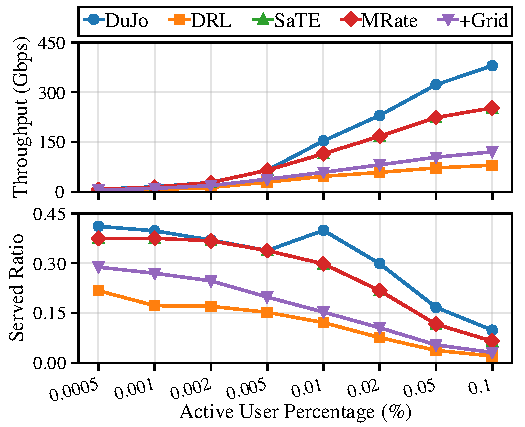
\includegraphics[scale=0.85]{plot_test_tcom_shell_time_load_scaling.pdf}
\caption{\blue{(Fig. \ref{fig:plot_test_tcom_shell_time_load_scaling} in the revised manuscript) Load-stress evaluation on the structured shell-based Starlink instance. The active-user percentage varies from $0.0005\%$ to $0.1\%$. The top and the bottom plots show the throughput and the served-demand ratio, respectively.}}
\label{fig:resp_plot_test_tcom_shell_time_load_scaling}
\end{figure}


\textbf{Comment 7: From a system level perspective, author should provide an idea of the operation of the system. Is the optimization carried out by the satellites or centrally orchestrated by a ground station?}

\textbf{Response:} We agree that the operating architecture should be stated explicitly. The present formulation is intended as a centrally orchestrated per-snapshot planner, carried out by the ground segment or network-control segment rather than independently by the satellites \cite{3gpp38821,guidotti2024role}. For each snapshot, the controller uses predicted ephemerides, gateway availability, and traffic estimates to compute the matching, routing, and rate-allocation decisions, and then disseminates the resulting schedule to the satellites for execution. We also added a short discussion of the main practical challenges that are abstracted away by this model, namely control-plane latency, imperfect traffic or state estimates, and robustness under snapshot-to-snapshot disturbances or link interruptions. We then stated that hierarchical or distributed implementations, together with robust or online re-optimization under delayed or imperfect state information, are natural future directions \cite{guidotti2024role,wu2025enhancing}.

\textbf{Manuscript changes:} In the system model section, we added a short paragraph that states the intended control architecture, clarifies that the current method is a centrally orchestrated planner rather than a distributed onboard optimization method, and briefly discusses real-world deployment challenges and future directions. The key revised text read as follows.

In Section~\ref{sec:system_model}, we stated:

``\dots\blue{From a system-operation perspective, the optimization is intended to be carried out centrally by the ground segment or network-control segment rather than independently onboard the satellites \cite{3gpp38821,guidotti2024role}. For each snapshot, the controller uses predicted ephemerides, gateway availability, and traffic estimates to compute the matching, routing, and rate-allocation decisions, and then disseminates the resulting schedule to the satellites for execution. In real deployments, this workflow would also face control-plane latency, imperfect traffic or state estimates, and robustness challenges under snapshot-to-snapshot disturbances or link interruptions \cite{guidotti2024role,wu2025enhancing}. Hierarchical or distributed implementations, together with robust or online re-optimization under delayed or imperfect state information, are therefore important future directions.}''

\textbf{Comment 8: Figure 2 is not very representative. It is not clear the comparison of b) and c).}

\textbf{Response:} We agree that the comparison between panels (b) and (c) should be stated more explicitly. We also agree that Fig.~\ref{fig:constellation_simulation_1000_compare} should be read as an illustrative snapshot rather than the main evidence for representativeness. The representative validation is provided by the quantitative structured-shell, load-stress, and multi-constellation results reproduced in this response letter. To address the clarity issue in Fig.~\ref{fig:constellation_simulation_1000_compare}, we revised its caption so that the roles of the three panels are stated directly. In particular, the revised caption now states that panel (a) shows the constellation snapshot together with the LISLs selected by DuJo, the user distribution, and the ground-gateway locations, while panels (b) and (c) show the same geographic zoom and the same traffic-demand snapshot under DuJo and MRate, respectively. We also stated explicitly that the inset boxes in panels (b) and (c) report the compared metrics, namely the number of connected flows, flow-path length, and net throughput.

\textbf{Manuscript changes:} We revised only the caption of Fig.~\ref{fig:constellation_simulation_1000_compare} so that the meaning of each panel and the comparison between panels (b) and (c) are stated directly. The revised caption read as follows.

``\blue{Comparison for the simulated Starlink-based constellation instance with $I=1000$ satellites. Panel (a) shows the constellation snapshot together with the LISLs selected by DuJo, the user distribution, and the ground-gateway locations. Panels (b) and (c) show the same geographic zoom and the same traffic-demand snapshot under DuJo and MRate, respectively, so their routed flow paths can be compared directly. The inset boxes in panels (b) and (c) report the resulting number of connected flows, flow-path length, and net throughput for the two schemes.}''

For direct inspection, the revised Fig. \ref{fig:constellation_simulation_1000_compare} is also reproduced in this response letter.

\begin{figure}[H]
\centering
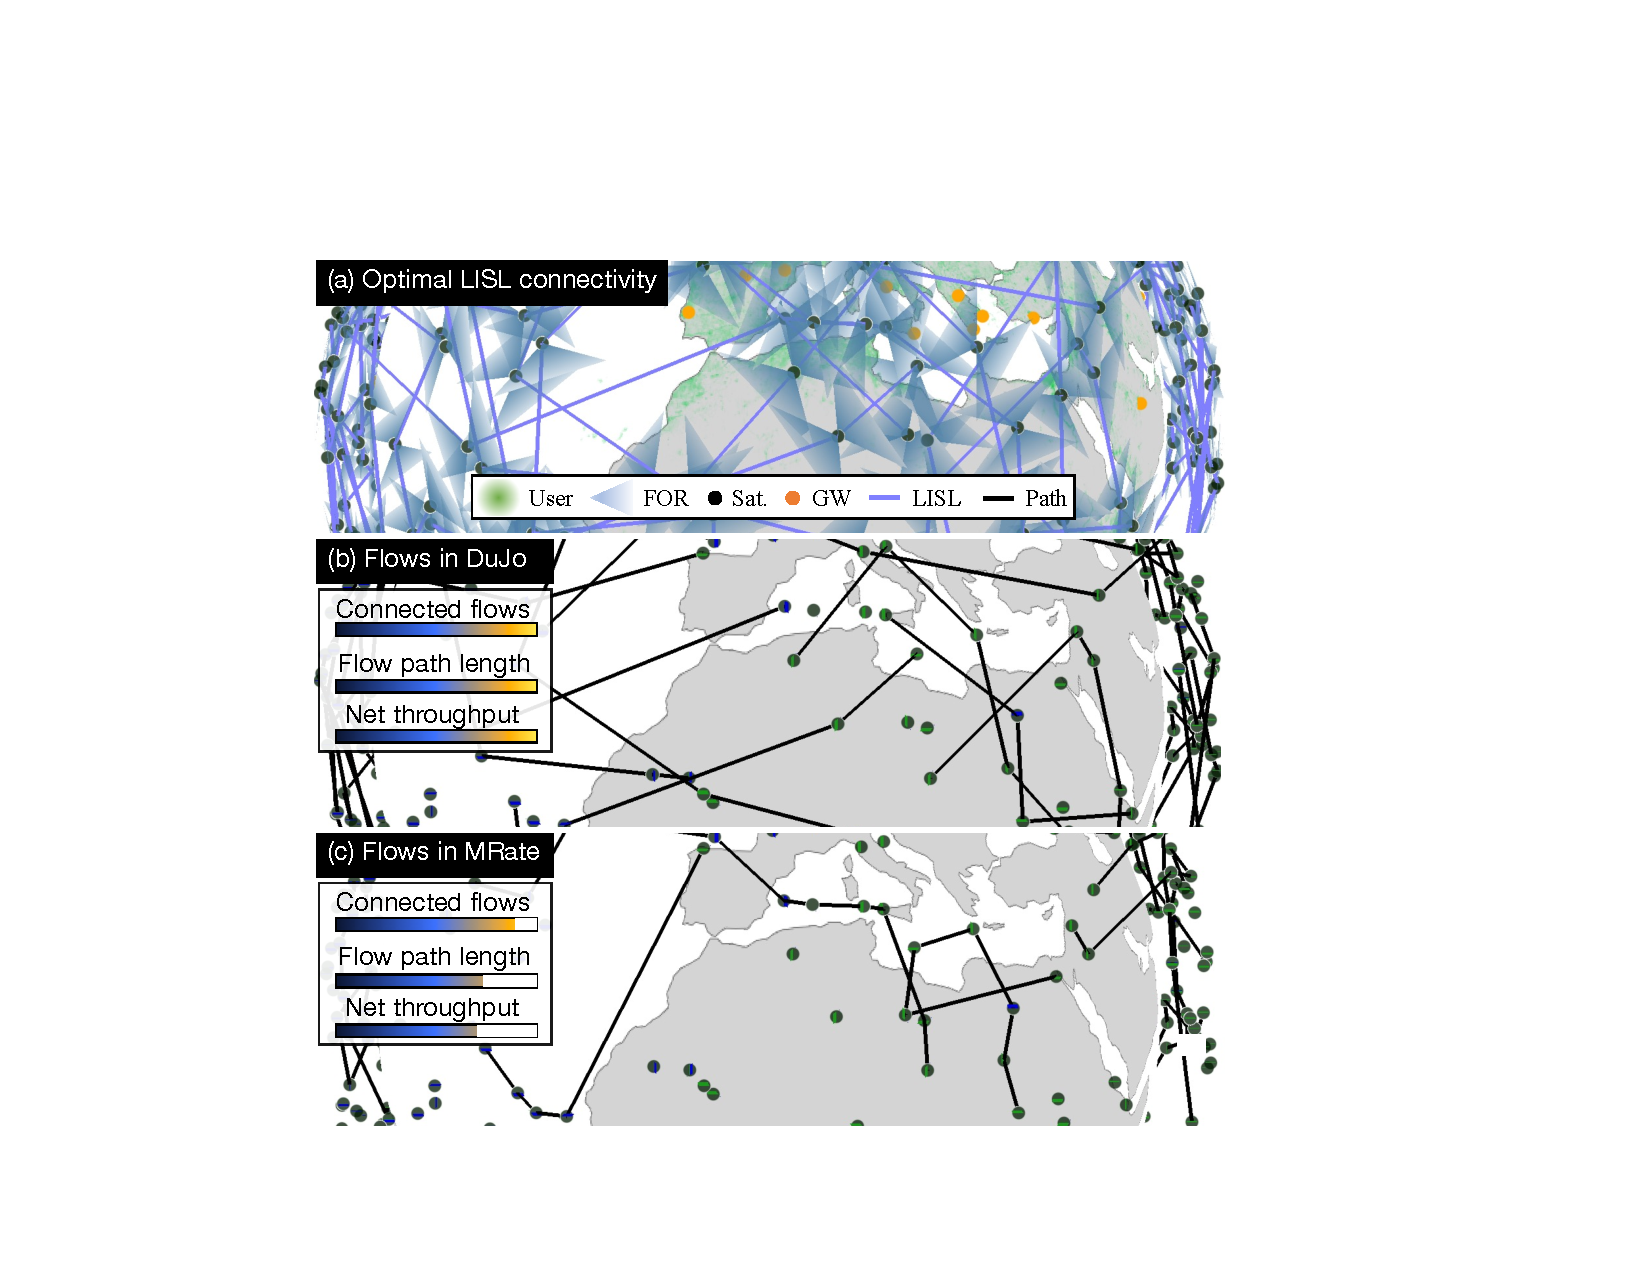
\includegraphics[width=.95\columnwidth]{constellation_simulation_1000_compare_rev.pdf}
\caption{\blue{(Fig. \ref{fig:constellation_simulation_1000_compare} in the revised manuscript) Comparison for the simulated Starlink-based constellation instance with $I=1000$ satellites. Panel (a) shows the constellation snapshot together with the LISLs selected by DuJo, the user distribution, and the ground-gateway locations. Panels (b) and (c) show the same geographic zoom and the same traffic-demand snapshot under DuJo and MRate, respectively, so their routed flow paths can be compared directly. The inset boxes in panels (b) and (c) report the resulting number of connected flows, flow-path length, and net throughput for the two schemes.}}
\label{fig:resp_constellation_simulation_1000_compare}
\end{figure}

\textbf{Comment 9: When modelling Starlink, authors select a random number of satellites out of the whole constellation. This might lead to unreal scenarios, without a reliable representation of potential ISLs between the selected satellites.}

\textbf{Response:} We agree that randomly selecting satellites from the whole Starlink constellation can produce unrealistic candidate-ISL geometry if it is treated as the main validation setting. In the revised manuscript, random Starlink subsets are therefore retained only for the varying-$I$ and computing-time sensitivity study, where the purpose is to test scaling with constellation size. The realism-oriented Starlink evaluation instead uses one coherent $I=1000$ satellite block from the dominant $53.2^\circ$ shell and tracks the same satellites over six snapshot times, so the selected satellites preserve structured orbital geometry. We also added structured-constellation comparisons for a regular Walker-delta case and the OneWeb constellation in Fig. \ref{fig:plot_test_dual_optimization_different_constellation}. Thus, the random-subset results are not used as the sole evidence for realistic Starlink ISL behavior.

\textbf{Manuscript changes:} In the simulation setup and the numerical-results discussion, we revised the text accordingly. The revised text read as follows.

In the simulation setup, we stated:

``\dots\blue{To study problem-scale sensitivity, we randomly select $I$ satellites out of the Starlink constellation for the varying-$I$ and computing-time results. We also test a structured shell-based Starlink instance with $I=1000$ satellites. Specifically, at $\mathcal{T}_0$ we select a coherent 1000-satellite block from the dominant $53.2^\circ$ shell and then keep the same satellites over snapshot offsets of $0$, $30$, $60$, $90$, $120$, and $180$ min.}''

In Subsubsection~\ref{subsubsec:structured_shell_time_evaluation}, we stated:

``\dots\blue{We next evaluate the structured shell-based Starlink instance. Fig.~\ref{fig:plot_test_tcom_shell_time_baselines} shows the results for the same $I=1000$ satellite block over six snapshot times.}''

For direct inspection, the revised Figs. \ref{fig:plot_test_tcom_shell_time_baselines} and \ref{fig:plot_test_dual_optimization_different_constellation} are also reproduced in this response letter.

\begin{figure}[H]
\centering
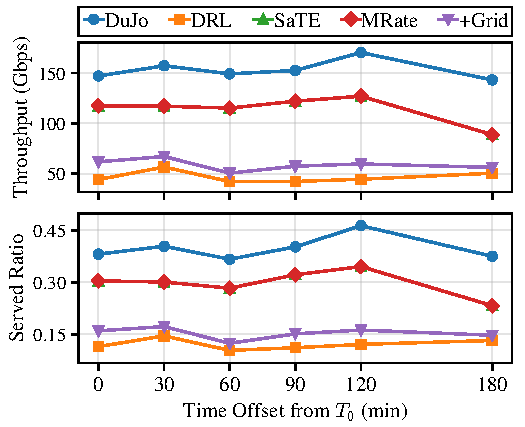
\includegraphics[scale=0.85]{plot_test_tcom_shell_time_baselines.pdf}
\caption{\blue{(Fig. \ref{fig:plot_test_tcom_shell_time_baselines} in the revised manuscript) Structured shell-based Starlink evaluation over time. A coherent $I=1000$ satellite block from the dominant $53.2^\circ$ shell is kept fixed while the constellation is propagated over snapshot offsets of $0$, $30$, $60$, $90$, $120$, and $180$ min. The top plot shows the served throughput and the bottom plot shows the served-demand ratio for DuJo, DRL, SaTE, MRate, and +Grid.}}
\label{fig:resp_plot_test_tcom_shell_time_baselines_r3c9}
\end{figure}

\begin{figure}[H]
\centering
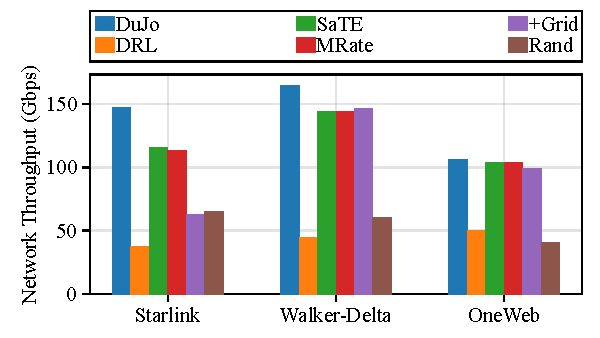
\includegraphics[scale=0.85]{plot_test_dual_optimization_different_constellation.pdf}
\caption{(Fig. \ref{fig:plot_test_dual_optimization_different_constellation} in the revised manuscript) Comparison in a Starlink-based ($I=1000$), a regular walker-delta ($50^{\circ}$ inclination, $I=1000$), and a OneWeb constellation ($I=650$).}
\label{fig:resp_plot_test_dual_optimization_different_constellation_r3c9}
\end{figure}

\textbf{Comment 10: A detailed analysis of the method performance in scenarios with a large traffic demand should be provided to have an idea of the resilience of the method.}

\textbf{Response:} We agree that resilience under higher offered load should be evaluated explicitly. In the revised manuscript, we therefore added a load-stress evaluation on the structured shell-based Starlink instance by varying the active-user percentage from $0.0005\%$ to $0.1\%$ while keeping the per-user demand fixed at $D=0.1$ Gbps. The added figure reports both the served throughput and the served-demand ratio, so the revised evaluation captures both throughput saturation and the shrinking served share in higher-load regimes. The resulting curves show that DuJo is strongest at all tested loads, while DRL remains below the heuristic baselines. For direct inspection, the revised Fig. \ref{fig:plot_test_tcom_shell_time_load_scaling} is also reproduced in this response letter.

\textbf{Manuscript changes:} In the simulation setup and the added load-stress subsection, we introduced the higher-load evaluation and the associated metrics. The key revised text read as follows.

In the simulation setup, we stated:

``\dots\blue{For the load-stress evaluation, we vary this active-user percentage from $0.0005\%$ to $0.1\%$ while keeping the user-demand model otherwise unchanged.}''

In Subsubsection~\ref{subsubsec:load_stress_evaluation}, we stated:

``\dots\blue{For the load-stress evaluation, we vary the active-user percentage while keeping the per-user demand fixed at $D=0.1$ Gbps. Fig.~\ref{fig:plot_test_tcom_shell_time_load_scaling} reports both the served throughput and the served-demand ratio.}''

``\dots\blue{As the active-user percentage increases, all methods carry more traffic in absolute terms, but the served-demand ratio also decreases, which indicates growing congestion in the gateway and LISL resources. DuJo is strongest at all tested loads. DRL remains below the heuristic baselines across this load range. This suggests that the joint optimization remains the most effective approach on this structured-shell benchmark, especially once the network becomes meaningfully loaded.}''


\bibliography{main}
\bibliographystyle{IEEEtran}

\end{document} 
